\section{Low Noise Figure Amplifier}

\subsection{Ideal Biasing}

In a similar manner as with the high gain amplifier I include below, in figures
\ref{fig:A2P2IdealSchematic} and \ref{fig:A2P2IdealBiasingResults},
respectively, the schematic and the results (scattering parameters and
stability) of the simulation at the design frequency (\SI{2}{\giga\hertz}).

Note that the stability parameters have been simulated in addition to having had
been calculated by hand (see the appendix for the relevant Mathematica code).
The two results for stability (simulation vs. hand calculations) are consistent
to within one part in a thousand (indicative of rounding errors).

\begin{figure}[H]
    \centering
    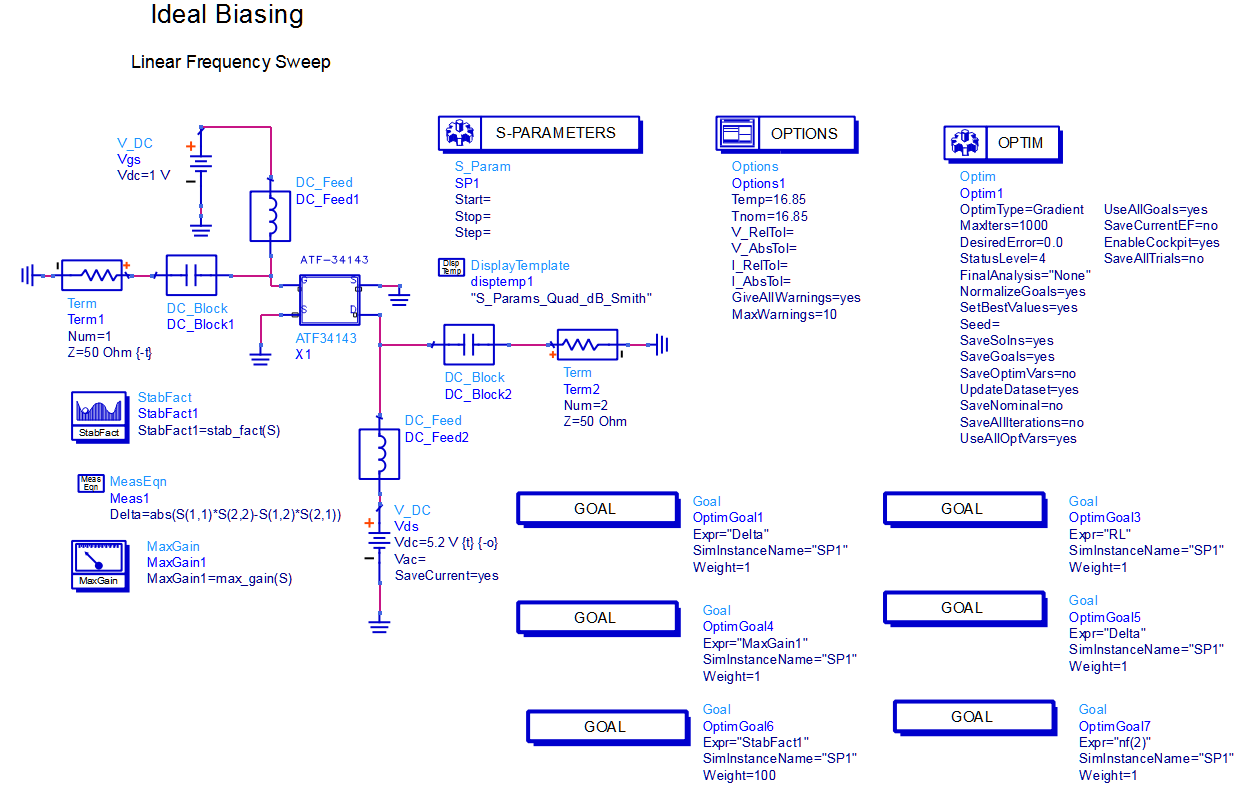
\includegraphics[width=0.8\linewidth]{Images/A2P2IdealSchematic.png}
    \caption{Schematic of the low noise amplifier ideal biasing network}
    \label{fig:A2P2IdealSchematic}
\end{figure}

\begin{figure}[H]
    \centering
    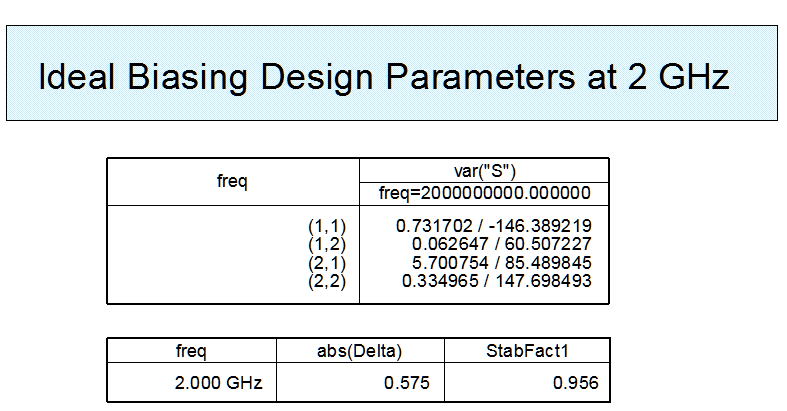
\includegraphics[width=0.8\linewidth]{Images/A2P2IdealBiasingResults.png}
    \caption{Results of the ADS simulation of the low noise amplifier ideal biasing network}
    \label{fig:A2P2IdealBiasingResults}
\end{figure}

\subsection{Physical Biasing}

The schematic and the simulation results of the physical biasing network for the
low noise amplifier are shown in figures \ref{fig:A2P2PhysicalSchematic} and
\ref{fig:A2P2PhysicalResults}, respectively.

Worthy of note: 
\begin{enumerate}
    \item   Figure \ref{fig:A2P2PhysicalResults} indicates stability over the
        entire bandwidth of consideration.
    \item   The maximum gain at the designed noise figure, $NF \approx
        \SI{.88}{\deci\bel}$, manages to be quite high at $\SI{2}{\giga\hertz}$:
        $G_{T_{max}} \approx \SI{16.8}{\deci\bel}$.
\end{enumerate}

\begin{figure}[H]
    \centering
    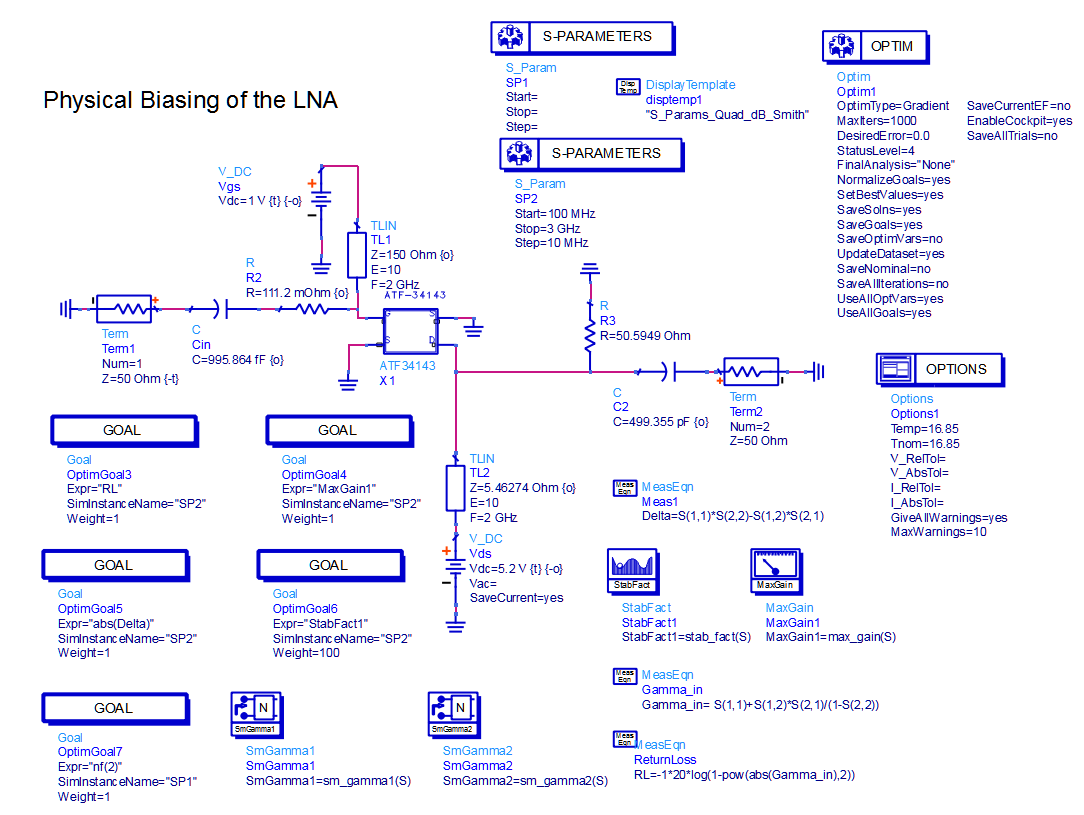
\includegraphics[width=0.8\linewidth]{Images/A2P2PhysicalSchematic.png}
    \caption{Schematic of the physical biasing network for the low noise
    amplifier.}
    \label{fig:A2P2PhysicalSchematic}
\end{figure}

\begin{figure}[H]
    \centering
    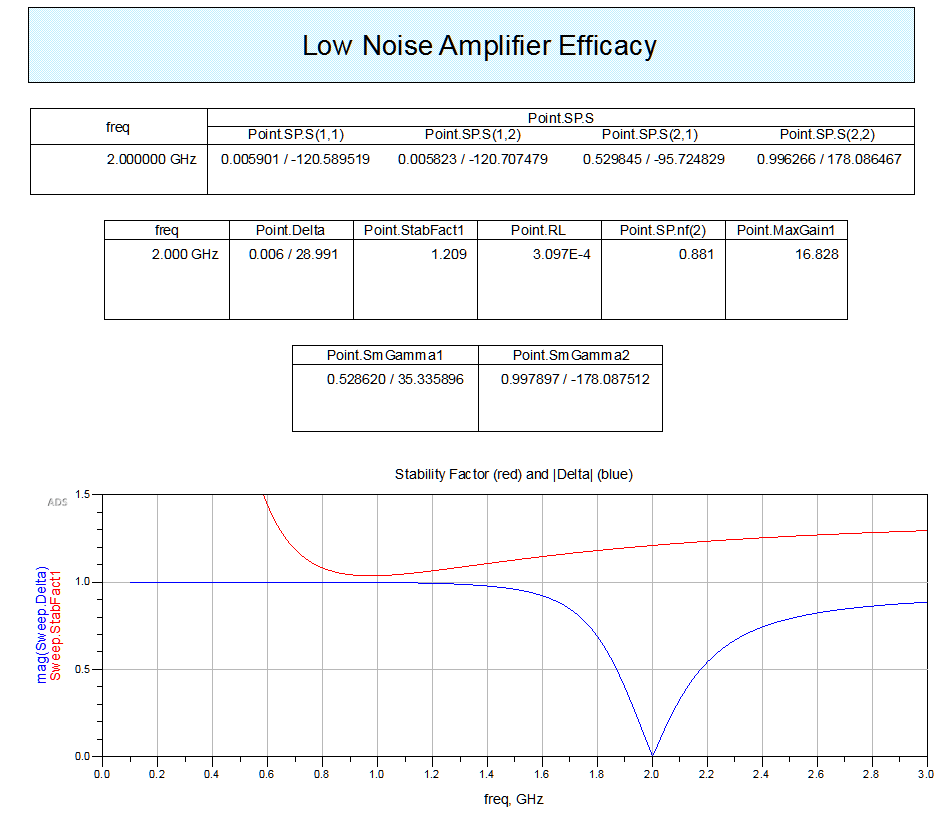
\includegraphics[width=0.8\linewidth]{Images/A2P2PhysicalResults.png}
    \caption{Efficacy of the low-noise amplifier physical biasing network.}
    \label{fig:A2P2PhysicalResults}
\end{figure}

\subsection{Low Noise Amplifier Design}

The full design for the low noise amplifier is shown in figure
\ref{fig:A2P2LNASchematic}. The design efficacy is demonstrated in figures
\ref{fig:A2P2LNADesignFrequencyEfficacy},
\ref{fig:A2P2LNAFrequencySweepStability} and \ref{fig:A2P2LNAFOM}. Note that the
desired gain of at least $\SI{15}{\deci\bel}$ has been achieved in addition to a
lower-than-desired noise figure of $\SI{.736}{\deci\bel}$. For reference, it is
shown in figure \ref{fig:A2P2LNADesignFrequencyEfficacy} that the input return
loss is $\approx \SI{28.30}{\deci\bel}$.

Note that there is also a non-negligible amount of mismatch shown between the
second terminal and the rest of the amplifier. I strongly believe that this is
due to numerical errors in the calculation of quantities used to determine
$\Gamma_{ml}$ within ADS. I have noticed many peculiar numerical errors. That I
should have recorded. For example, more than once, the ADS calculation of
$\Delta$ differed from values obtained by calculating $\Delta$ in Mathematica.
This is not a difficult calculation and ADS and Mathematica did agree for many
sets of scattering parameters. However, I have noticed many times that ADS does
not always report the same values obtained by using other calculators (the
values differ by as much as 30 percent).

\begin{figure}[H]
    \centering
    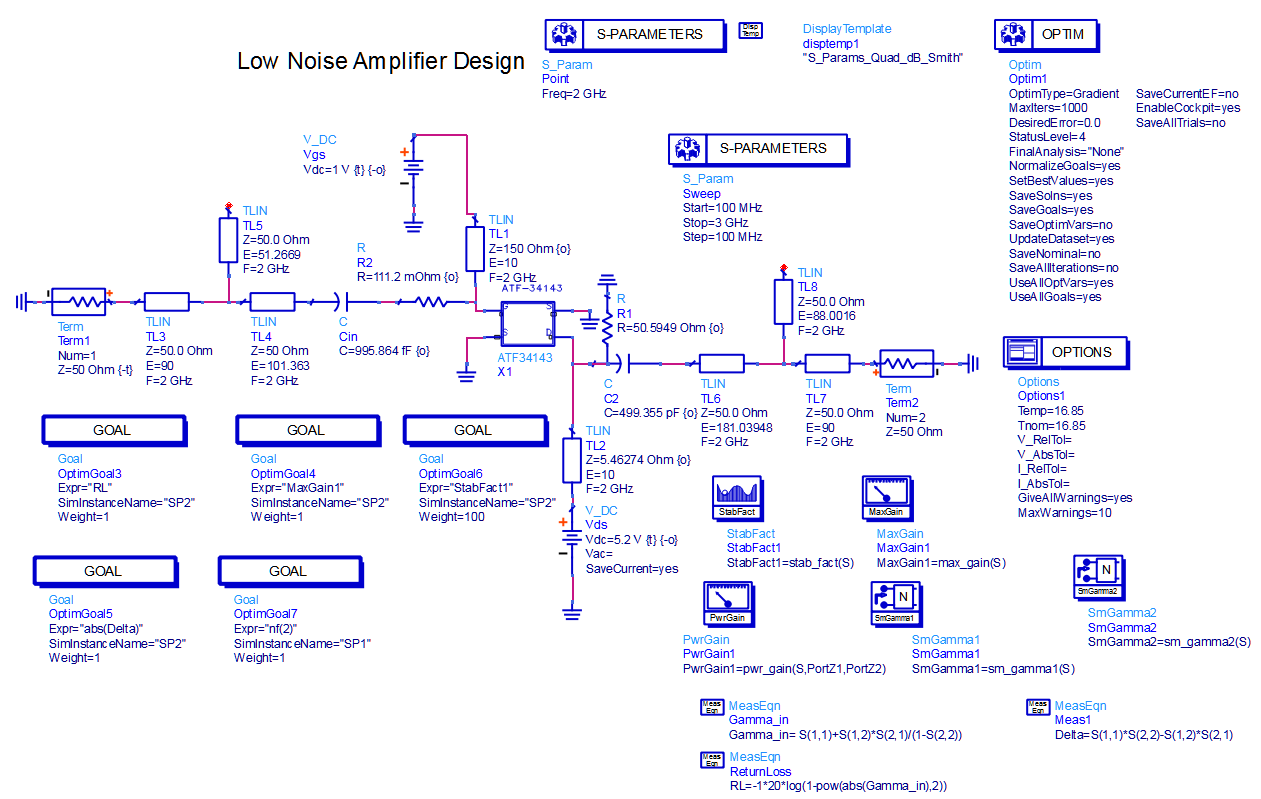
\includegraphics[width=0.8\linewidth]{Images/A2P2LNASchematic.png}
    \caption{Schematic of the LNA design.}
    \label{fig:A2P2LNASchematic}
\end{figure}

\begin{figure}[H]
    \centering
    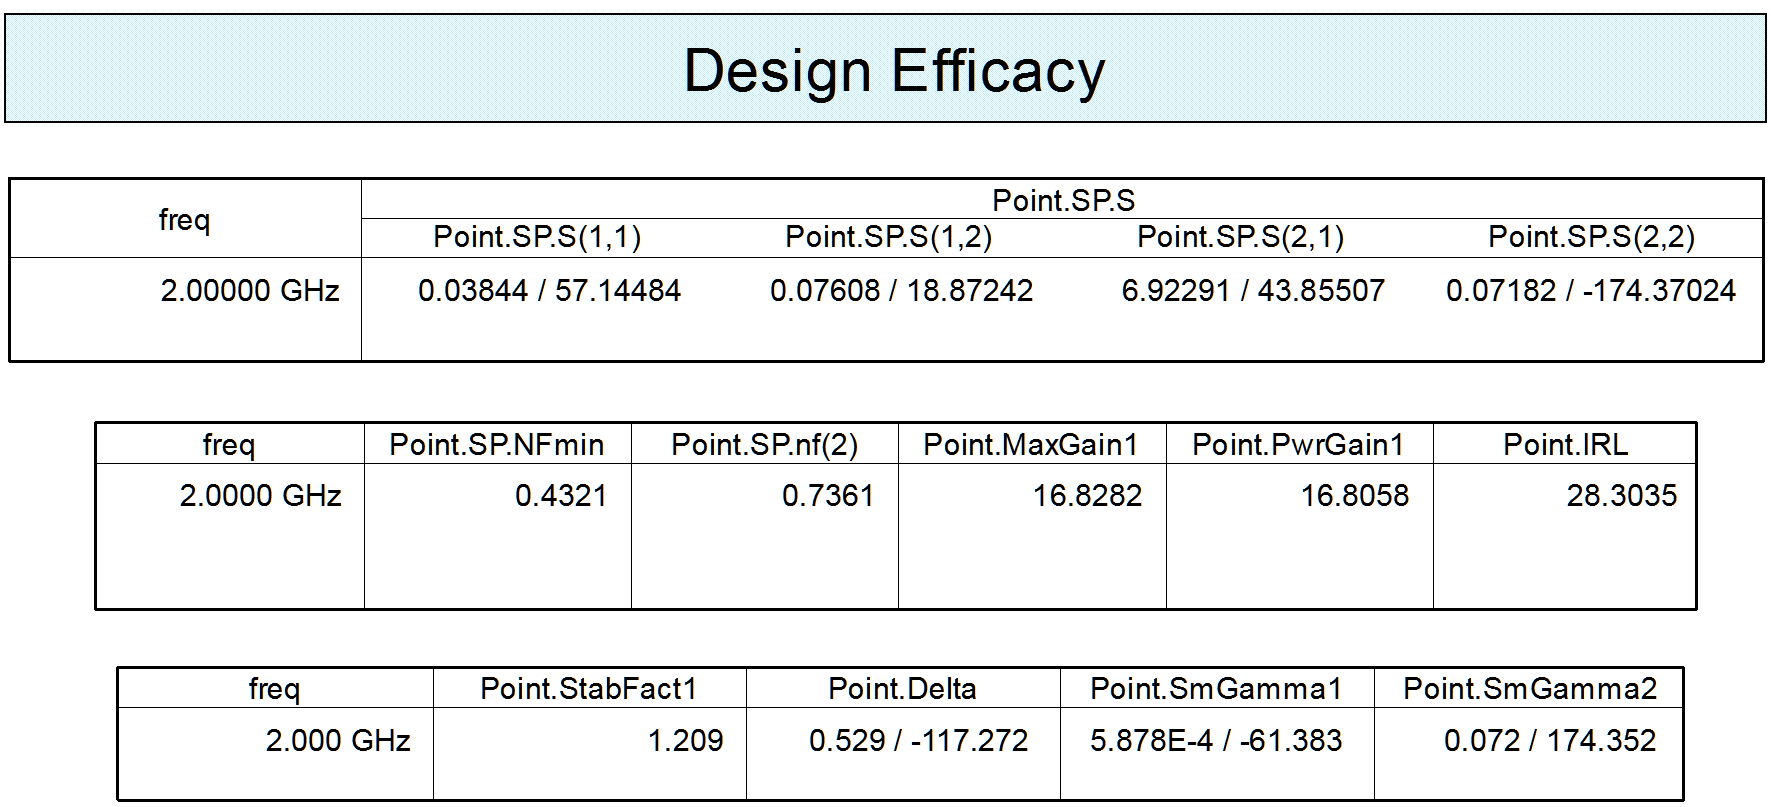
\includegraphics[width=0.8\linewidth]{Images/A2P2LNADesignFrequencyEfficacy.png}
    \caption{LNA efficacy at the design frequency: $\SI{2}{\giga\hertz}$.}
    \label{fig:A2P2LNADesignFrequencyEfficacy}
\end{figure}

\begin{figure}[H]
    \centering
    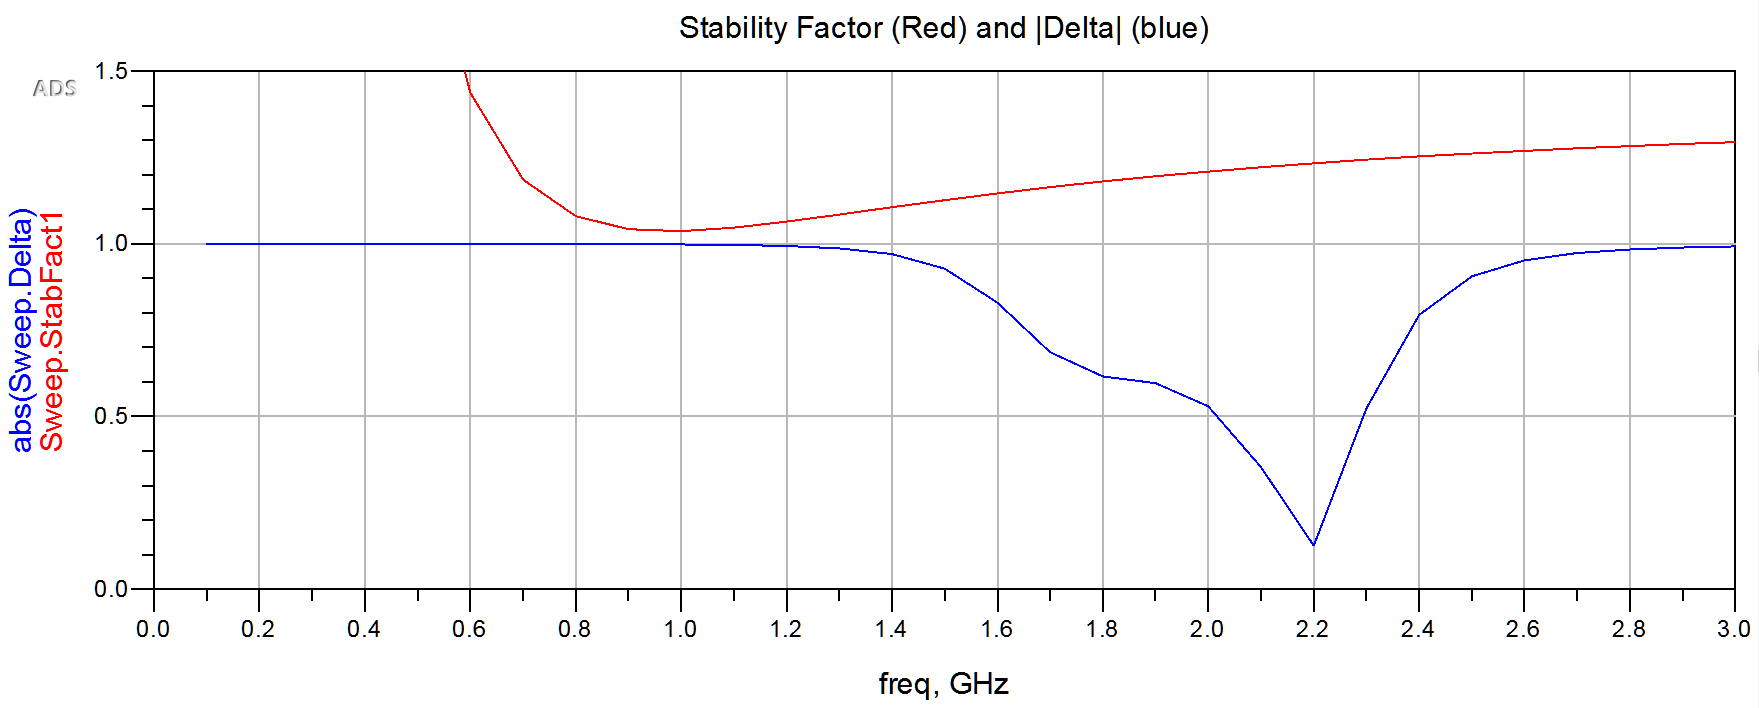
\includegraphics[width=0.8\linewidth]{Images/A2P2LNAFrequencySweepStability.png}
    \caption{LNA stability over the specified bandwidth of the amplifier.}
    \label{fig:A2P2LNAFrequencySweepStability}
\end{figure}

\begin{figure}[H]
    \centering
    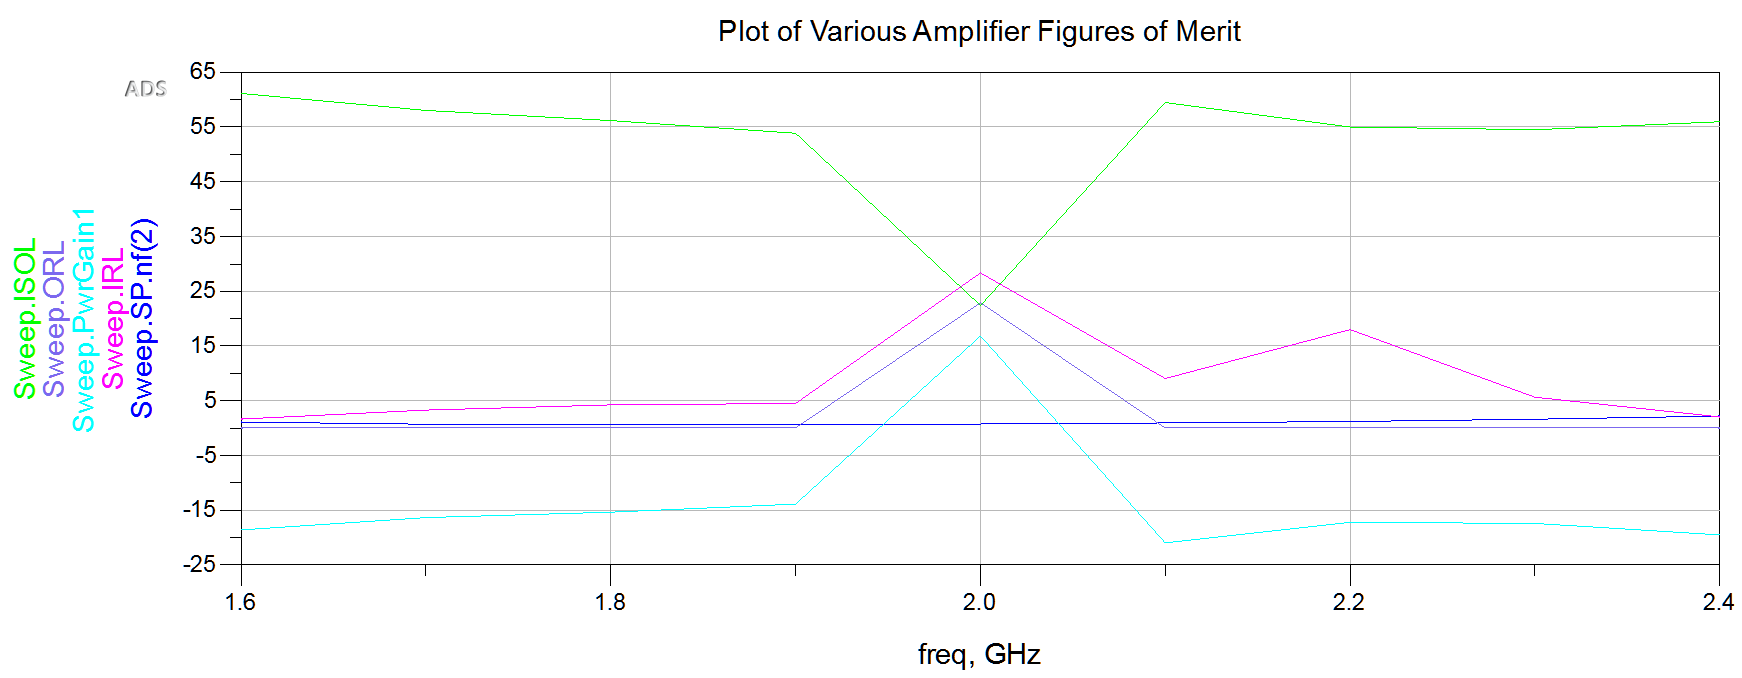
\includegraphics[width=0.8\linewidth]{Images/A2P2LNAFOM.png}
    \caption{Plot of various figures of merit of the amplifier including:
    Isolation (green), output return loss (purple), power gain (teal), input
return loss (pink) and noise figure (blue)}
    \label{fig:A2P2LNAFOM}
\end{figure}

